\section{Graph convolutional neural network (HAR)}

\subsection{Skeleton Graph Construction}
\begin{frame}{Skeleton Graph Construction}
    \begin{multicols} {2}
        \begin{enumerate}
            \item $V = \{v_{ti} | t = 1,...,T; i = 1,...,N\}$
                  \begin{itemize}
                      \item T is the number of frames
                      \item N is the number of joints
                  \end{itemize}
            \item $E_S = \{v_{ti}v_{tj} | (i, j) \in H\}$
                  \begin{itemize}
                      \item H is the set of naturally connected human body joints
                  \end{itemize}
            \item $E_F = \{v_{ti}v_{(t+1)i}\}$
        \end{enumerate}

        \begin{figure}[htp]
            \centering
            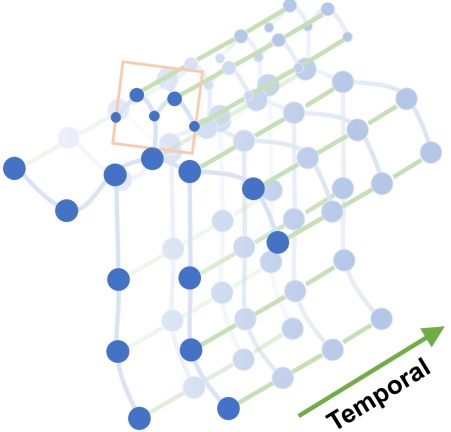
\includegraphics[width=0.4\textwidth]{topics/201031-yan2018spatial/assets/img/skeleton-st-graph.png}
            \caption{Skeleton Graph}
            \label{fig:skeleton-graph}
        \end{figure}
    \end{multicols}
\end{frame}

\subsection{Spatial Graph Convolutional Neural Network}
\begin{frame}{Spatial Graph Convolutional Neural Network}
    \begin{block}{Graph convolutional operation}
        $$f_{out}(v_{ti}) = \frac{1}{|B(v_{ti})|} \sum_{v_{tj} \in B(v_{ti})} f_{in}(v_{tj}) \times w(l_{ti}(v_{tj}))$$
        \begin{itemize}
            \item $B(v_{ti}) = \{v_{tj} | d(v_{ti}, v_{tj}) <= D\}$ (In this work we use D = 1)
            \item $w$ is the weight function provides a weight vector.
            \item $l_{ti}$ is the partitioning function.
        \end{itemize}
    \end{block}
\end{frame}

\begin{frame}{Spatial Graph Convolutional Neural Network}
    Several partition strategies: b) Uni-labeling, c) Distance partitioning, d) Spatial configuration partitioning.
    \begin{figure}[htp]
        \centering
        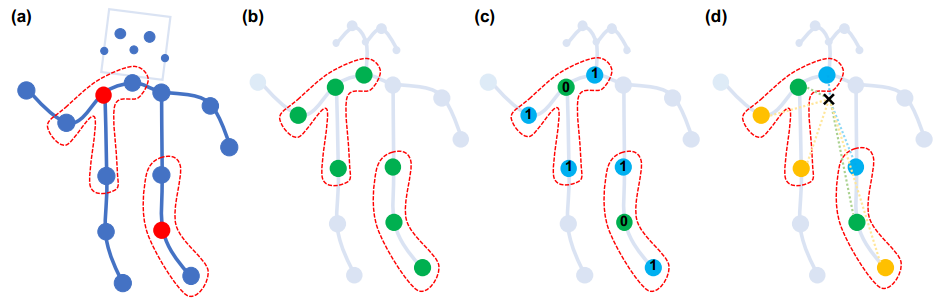
\includegraphics[width=0.7\textwidth]{topics/201031-yan2018spatial/assets/img/gcn-partition.png}
        \caption{Partition Strategies}
        \label{fig:partition-strategies}
    \end{figure}
\end{frame}
